\chapter{Time series filters}
\label{chap:tsfilter}

In addition to the usual application of lags and differences,
gretl provides fractional differencing and various filters
commonly used in macroeconomics for trend-cycle decomposition: notably
the Hodrick--Prescott filter \citep{hodrick97}, the Baxter--King
bandpass filter \citep{baxter-king99} and the Butterworth
filter \citep{butterworth30}.

\section{Fractional differencing}
\label{sec:fracdiff}

The concept of differencing a time series $d$ times is pretty obvious
when $d$ is an integer; it may seem odd when $d$ is
fractional. However, this idea has a well-defined mathematical
content: consider the function
\[
  f(z) = (1 - z)^{-d},
\]
where $z$ and $d$ are real numbers. By taking a Taylor series
expansion around $z=0$, we see that
\[
  f(z) = 1 + dz + \frac{d (d+1)}{2} z^2 + \cdots 
\]
or, more compactly,
\[
  f(z) = 1 + \sum_{i=1}^{\infty} \psi_i z^i
\]
with
\[
  \psi_k = \frac{\prod_{i=1}^{k} (d+i-1) }{k!} = \psi_{k-1} \frac{d+k-1}{k}
\]

The same expansion can be used with the lag operator, so that if we defined
\[
  Y_t = (1-L)^{0.5} X_t
\]
this could be considered shorthand for
\[
Y_t = X_t - 0.5 X_{t-1} - 0.125 X_{t-2} - 0.0625 X_{t-3} - \cdots 
\]
    
In gretl this transformation can be accomplished by the syntax 
\begin{code}
genr Y = fracdiff(X,0.5)
\end{code}

\section{The Hodrick--Prescott filter}
\label{sec:hodrick-prescott}

This filter is accessed using the \verb+hpfilt()+ function, which
takes as its first argument the name of the variable to be processed.
(Further optional arguments are explained below.)

A time series $y_t$ may be decomposed into a trend or growth
component $g_t$ and a cyclical component $c_t$.  
%
\[
y_t = g_t + c_t, \quad t = 1,2,\dots,T
\]
%
The Hodrick--Prescott filter effects such a decomposition by
minimizing the following:
%
\[
    \sum_{t = 1}^T {(y_t - g_t )^2 } + \lambda \sum_{t = 2}^{T -
      1} \left((g_{t+1} - g_t) - (g_t - g_{t - 1} )\right)^2 .
\]
%
The first term above is the sum of squared cyclical components $c_t =
y_t - g_t$. The second term is a multiple $\lambda$ of the sum of
squares of the trend component's second differences. This
second term penalizes variations in the growth rate of the trend
component: the larger the value of $\lambda$, the higher is the
penalty and hence the smoother the trend series.

Note that the \cmd{hpfilt} function in gretl produces the
cyclical component, $c_t$, of the original series.  If you want the
smoothed trend you can subtract the cycle from the original:

\begin{code}
genr ct = hpfilt(yt)
genr gt = yt - ct
\end{code}

\cite{hodrick97} suggest that a value of $\lambda = 1600$ is reasonable
for quarterly data.  The default value in gretl is 100 times the
square of the data frequency (which, of course, yields 1600 for
quarterly data).  The value can be adjusted using an optional
second argument to \verb+hpfilt()+, as in
%
\begin{code}
genr ct = hpfilt(yt, 1300)
\end{code}

As of version 2018a, the \cmd{hpfilt()} function accepts a third,
optional Boolean argument. If set to non-zero, what is performed is
the so-called \emph{one-sided} version of the filter. See Section
\ref{sec:example_hp} for further details.

\section{The Baxter and King filter}
\label{sec:baxter-king}

This filter is accessed using the \verb+bkfilt()+ function, which
again takes the name of the variable to be processed as its first
argument. The operation of the filter can be controlled via three
further optional argument.

Consider the spectral representation of a time series $y_t$:
%       
\[ y_t = \int_{-\pi}^{\pi} e^{i\omega} \mathrm{d} Z(\omega) \]
%
To extract the component of $y_t$ that lies between the frequencies
$\underline{\omega}$ and $\overline{\omega}$ one could apply a
bandpass filter:
%       
\[ c^*_t = \int_{-\pi}^{\pi} F^*(\omega) e^{i\omega} \mathrm{d}
Z(\omega) \]
%
where $F^*(\omega) = 1$ for $\underline{\omega} < |\omega| <
\overline{\omega}$ and 0 elsewhere. This would imply, in the time
domain, applying to the series a filter with an infinite number of
coefficients, which is undesirable. The Baxter and King bandpass
filter applies to $y_t$ a finite polynomial in the lag
operator $A(L)$:
%       
\[ c_t = A(L) y_t \]
%
where $A$($L$) is defined as
%       
\[ A(L) = \sum_{i=-k}^{k} a_i L^i \]

The coefficients $a_i$ are chosen such that $F(\omega)
= A(e^{i\omega})A(e^{-i\omega})$ is the best approximation to
$F^*(\omega)$ for a given $k$. Clearly, the higher $k$ the better the
approximation is, but since $2k$ observations have to be discarded, a
compromise is usually sought. Moreover, the filter has also other
appealing theoretical properties, among which the property that $A(1)
= 0$, so a series with a single unit root is made stationary by
application of the filter.

In practice, the filter is normally used with monthly or quarterly
data to extract the ``business cycle'' component, namely the component
between 6 and 36 quarters. Usual choices for $k$ are 8 or 12 (maybe
higher for monthly series).  The default values for the frequency
bounds are 8 and 32, and the default value for the approximation
order, $k$, is 8. You can adjust these values using the full form
of \verb+bkfilt()+, which is

\texttt{bkfilt(}\textsl{seriesname}\texttt{,} \textsl{f1}\texttt{,} 
 \textsl{f2}\texttt{,} \textsl{k}\texttt{)}

where \textsl{f1} and \textsl{f2} represent the lower and upper
frequency bounds respectively.

\section{The Butterworth filter}
\label{sec:butterworth}

The Butterworth filter \citep{butterworth30} is an approximation to an
``ideal'' square-wave filter. The ideal filter divides the spectrum of
a time series into a pass-band (frequencies less than some chosen
$\omega^{\star}$ for a low-pass filter, or frequencies greater than
$\omega^{\star}$ for high-pass) and a stop-band; the gain is 1 for the
pass-band and 0 for the stop-band. The ideal filter is unattainable in
practice since it would require an infinite number of coefficients,
but the Butterworth filter offers a remarkably good
approximation. This filter is derived and persuasively advocated by
\cite{pollock2000}.

For data $y$, the filtered sequence $x$ is given by
%
\begin{equation}
\label{eq:butter}
x = y - \lambda \Sigma Q(M + \lambda Q'\Sigma Q)^{-1}Q'y
\end{equation}
%
where
\[
\Sigma = \{2I_T - (L_T +  L^{-1}_T)\}^{T-2}
\quad \mbox{and} \quad
M =   \{2I_T + (L_T +  L^{-1}_T)\}^{T}
\]
%
$I_T$ denotes the identity matrix of order $T$; $L_T = [e_1, e_2,
\ldots, e_{T-1}, 0]$ is the finite-sample matrix version of the lag
operator; and $Q$ is defined such that pre-multiplication of a
$T$-vector of data by $Q'$ of order $(T-2) \times T$ produces the
second differences of the data. The matrix product
\[
Q'\Sigma Q = \{2I_T - (L_T +  L^{-1}_T)\}^{T}
\]
is a Toeplitz matrix.

The behavior of the Butterworth filter is governed by two parameters:
the frequency cutoff $\omega^{\star}$ and an integer order, $n$, which
determines the number of coefficients used. The $\lambda$ that appears
in (\ref{eq:butter}) is $\tan(\omega^{\star}/2)^{-2n}$.  Higher
values of $n$ produce a better approximation to the ideal filter in
principle (i.e.\ a sharper cut between the pass-band and the
stop-band) but there is a downside: with a greater number of
coefficients numerical instability may be an issue, and the influence
of the initial values in the sample may be exaggerated.

In gretl the Butterworth filter is implemented by the
\verb+bwfilt()+ function,\footnote{The code for this filter is based
  on D. S. G. Pollock's programs \app{IDEOLOG} and \app{DETREND}. The
  Pascal source code for the former is available from
  \url{http://www.le.ac.uk/users/dsgp1} and the C sources for the
  latter were kindly made available to us by the author.} which takes
three arguments: the series to filter, the order $n$ and the frequency
cutoff, $\omega^{\star}$, expressed in degrees. The cutoff value must
be greater than 0 and less than 180. This function operates as a
low-pass filter; for the high-pass variant, subtract the filtered
series from the original, as in
%
\begin{code}
series bwcycle = y - bwfilt(y, 8, 67)
\end{code}

Pollock recommends that the parameters of the Butterworth filter be
tuned to the data: one should examine the periodogram of the series in
question (possibly after removal of a polynomial trend) in search of a
``dead spot'' of low power between the frequencies one wishes to
exclude and the frequencies one wishes to retain. If $\omega^{\star}$
is placed in such a dead spot then the job of separation can be done
with a relatively small $n$, hence avoiding numerical problems. By way
of illustration, consider the periodogram for quarterly observations
on new cars sales in the US,\footnote{This is the variable
  \texttt{QNC} from the Ramanathan data file \texttt{data9-7}.} 1975:1
to 1990:4 (the upper panel in Figure~\ref{fig:QNCfilt}).

\begin{figure}[htbp]
  \centering
 \begin{tabular}{cc}
  \multicolumn{2}{c}{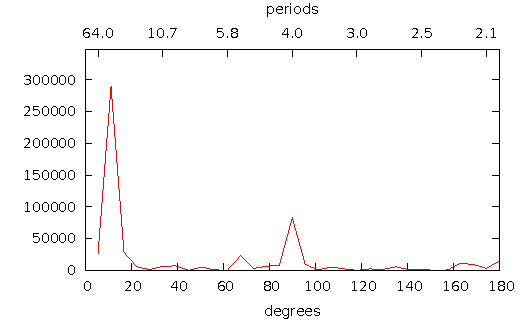
\includegraphics[scale=0.85]{figures/QNCpergm}} \\
  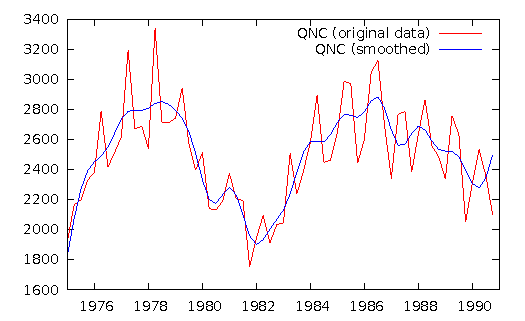
\includegraphics[scale=0.85]{figures/QNCfilt} &
\vbox{\hbox{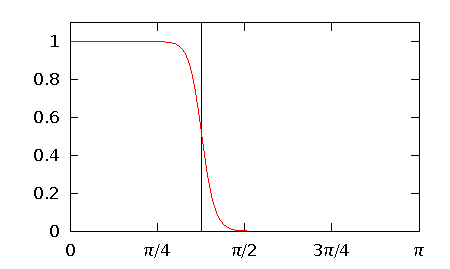
\includegraphics[scale=0.8]{figures/filtergain}}\vskip .3in}
\end{tabular}
\caption{The Butterworth filter applied}
\label{fig:QNCfilt}
\end{figure}

A seasonal pattern is clearly visible in the periodogram, centered at
an angle of 90$^{\circ}$ or 4 periods. If we set $\omega^{\star} =
68^{\circ}$ (or thereabouts) we should be able to excise the
seasonality quite cleanly using $n=8$.  The result is shown in the
lower panel of the Figure, along with the frequency response or gain
plot for the chosen filter. Note the smooth and reasonably steep
drop-off in gain centered on the nominal cutoff of $68^{\circ} \approx
3\pi/8$.

The apparatus that supports this sort of analysis in the gretl
GUI can be found under the \textsf{Variable} menu in the main window:
the items \textsf{Periodogram} and \textsf{Filter}. In the periodogram
dialog box you have the option of expressing the frequency axis in
degrees, which is helpful when selecting a Butterworth filter; and in
the Butterworth filter dialog you have the option of plotting the
frequency response as well as the smoothed series and/or the residual
or cycle.

\section{The discrete Fourier transform}
\label{sec:genr-fft} % Moved here from the genr chapter, thus this label.

The Fourier transform is not itself a time-series filter, but by providing
the bridge between the time and the frequency domain it is a fundamental
building block of many filter internals and deserves some detailed
comments.

The discrete Fourier transform can be best thought of as a linear,
invertible transform of a complex vector. Hence, if $\mathbf{x}$ is an
$n$-dimensional vector whose $k$-th element is $x_k = a_k + i b_k$,
then the output of the discrete Fourier transform is a vector
$\mathbf{f} = \mathcal{F}(\mathbf{x})$ whose $k$-th element is
\[
  f_k = \sum_{j=0}^{n-1} e^{-i \omega(j,k) } x_j
\]
where $\omega(j,k) = 2 \pi i \frac{j k}{n}$. Since the transformation
is invertible, the vector $\mathbf{x}$ can be recovered from
$\mathbf{f}$ via the so-called inverse transform
\[
  x_k = \frac{1}{n} \sum_{j=0}^{n-1} e^{i \omega(j,k) } f_j .
\]

The Fourier transform is used in many diverse situations
on account of this key property: the convolution of two vectors can be
performed efficiently by multiplying the elements of their Fourier
transforms and inverting the result.  If
\[
  z_k = \sum_{j=1}^n x_j y_{k-j} ,
\]
then
\[
  \mathcal{F}(\mathbf{z}) = \mathcal{F}(\mathbf{x}) \odot
  \mathcal{F}(\mathbf{y}) .
\]
That is, $\mathcal{F}(\mathbf{z})_k = \mathcal{F}(\mathbf{x})_k
\mathcal{F}(\mathbf{y})_k$.

For computing the Fourier transform, gretl uses the external
library \texttt{fftw3}: see \cite{frigo05}. This guarantees
extreme speed and accuracy. In fact, the CPU time needed to perform
the transform is $O(n \log n)$ for any $n$. This is why the array of
numerical techniques employed in \texttt{fftw3} is commonly known as
the \emph{Fast} Fourier Transform.

gretl provides two matrix functions for performing the Fourier transform
and its inverse: \texttt{fft} and \texttt{ffti}.\footnote{The function 
\texttt{fft} predates gretl's native support of complex matrices and 
returns the real and imaginary parts of the result in separate columns,
as described below. For new scripts it is recommended to use the newer
function \texttt{fft2} instead, which will return a complex matrix of 
the same dimension as the input. But the meaning and semantics are the 
same. The inverse function \texttt{ffti} supports both representations.}
In fact, gretl's
implementation of the Fourier transform is somewhat more specialized:
the input to the \texttt{fft} function is understood to be real.
Conversely, \texttt{ffti} takes a complex argument and delivers a real
result. For example:
\begin{code}
matrix x1 = { 1 ; 2 ; 3 }
# perform the transform
matrix f = fft(x1)
# perform the inverse transform
matrix x2 = ffti(f)
\end{code}
yields
\[
  x_1 = \left[ \begin{array}{c} 1 \\ 2 \\ 3 \end{array} \right]
  \qquad
  f = \left[ \begin{array}{rr}
      6 & 0 \\ -1.5 & 0.866 \\ -1.5 & -0.866
   \end{array} \right]
  \qquad
  x_2 = \left[ \begin{array}{c} 1 \\ 2 \\ 3 \end{array} \right]
\]
where the first column of \emph{f} holds the real part and the second
holds the complex part. In general, if the input to \texttt{fft} has
$n$ columns, the output has $2n$ columns, where the real parts are
stored in the odd columns and the complex parts in the even
ones. Should it be necessary to compute the Fourier transform on
several vectors with the same number of elements, it is numerically more
efficient to group them into a matrix rather than invoking
\texttt{fft} for each vector separately.

As an example, consider the multiplication of two polynomials:
\begin{eqnarray*}
  a(x) & = & 1 + 0.5 x \\
  b(x) & = & 1 + 0.3 x - 0.8 x^2 \\
  c(x) = a(x) \cdot b(x) & = & 1 + 0.8 x - 0.65 x^2 - 0.4 x^3
\end{eqnarray*}
The coefficients of the polynomial $c(x)$ are the convolution of the
coefficients of $a(x)$ and $b(x)$; the following gretl code fragment
illustrates how to compute the coefficients of $c(x)$:
\begin{code}
# define the two polynomials
a = { 1, 0.5, 0, 0 }'
b = { 1, 0.3, -0.8, 0 }'
# perform the transforms
fa = fft(a)
fb = fft(b)
# complex-multiply the two transforms
fc = cmult(fa, fb)
# compute the coefficients of c via the inverse transform
c = ffti(fc)
\end{code}

Maximum efficiency would have been achieved by grouping \texttt{a} and
\texttt{b} into a matrix.  The computational advantage is so little in
this case that the exercise is a bit silly, but the following
alternative may be preferable for a large number of
rows/columns:
\begin{code}
# define the two polynomials
a = { 1 ; 0.5; 0 ; 0 }
b = { 1 ; 0.3 ; -0.8 ; 0 }
# perform the transforms jointly
f = fft(a ~ b)
# complex-multiply the two transforms
fc = cmult(f[,1:2], f[,3:4])
# compute the coefficients of c via the inverse transform
c = ffti(fc)
\end{code}

Traditionally, the Fourier transform in econometrics has been mostly
used in time-series analysis, the periodogram being the best known
example. Listing~\ref{scr:pergm-fft} shows how to compute the
periodogram of a time series via the \texttt{fft} function.

\begin{script}[htbp]
  \scriptcaption{Periodogram via the Fourier transform}
  \label{scr:pergm-fft}
\begin{scode}
nulldata 50
# generate an AR(1) process
series e = normal()
series x = 0
x = 0.9*x(-1) + e
# compute the periodogram
scale = 2*$pi*$nobs
X = {x}
F = fft(X)
S = sumr(F.^2)
S = S[2:($nobs/2)+1]/scale
omega = seq(1,($nobs/2))' .* (2*$pi/$nobs)
omega = omega ~ S
# compare the built-in command
pergm x
print omega
\end{scode}
\end{script}

%%% Local Variables: 
%%% mode: latex
%%% TeX-master: "gretl-guide"
%%% End: 
